\documentclass[
11pt, % The default document font size, options: 10pt, 11pt, 12pt
%codirector, % Uncomment to add a codirector to the title page
]{charter} 




% El títulos de la memoria, se usa en la carátula y se puede usar el cualquier lugar del documento con el comando \ttitle
\titulo{Sistema de monitoreo y control de ambientes a distancia} 

% Nombre del posgrado, se usa en la carátula y se puede usar el cualquier lugar del documento con el comando \degreename
%\posgrado{Carrera de Especialización en Sistemas Embebidos} 
\posgrado{Carrera de Especialización en Internet de las Cosas} 
%\posgrado{Carrera de Especialización en Intelegencia Artificial}
%\posgrado{Maestría en Sistemas Embebidos} 
%\posgrado{Maestría en Internet de las cosas}

% Tu nombre, se puede usar en cualquier lugar del documento con el comando \authorname
\autor{Ing. César Javier Fanelli} 

% El nombre del director y co-director, se puede usar el cualquier lugar del documento con el comando \supname y \cosupname y \pertesupname y \pertecosupname
\director{Ing. Fernando Lichtschein}
\pertenenciaDirector{FIUBA} 
% FIXME:NO IMPLEMENTADO EL CODIRECTOR ni su pertenencia
\codirector{Ing. María Celeste Corominas} % para que aparezca en la portada se debe descomentar la opción codirector en el documentclass
\pertenenciaCoDirector{FIUBA}

% Nombre del cliente, quien va a aprobar los resultados del proyecto, se puede usar con el comando \clientename y \empclientename
\cliente{Mg. Ing. Damián Corbalán}
\empresaCliente{Movistar}

% Nombre y pertenencia de los jurados, se pueden usar el cualquier lugar del documento con el comando \jurunoname, \jurdosname y \jurtresname y \perteunoname, \pertedosname y \pertetresname.
\juradoUno{Nombre y Apellido (1)}
\pertenenciaJurUno{pertenencia (1)} 
\juradoDos{Nombre y Apellido (2)}
\pertenenciaJurDos{pertenencia (2)}
\juradoTres{Nombre y Apellido (3)}
\pertenenciaJurTres{pertenencia (3)}
 
\fechaINICIO{21 de octubre de 2022}		%Fecha de inicio de la cursada de GdP \fechaInicioName
\fechaFINALPlan{8 de diciembre de 2022} 	%Fecha de final de cursada de GdP
\fechaFINALTrabajo{a definir}	%Fecha de defensa pública del trabajo final


\begin{document}

\maketitle
\thispagestyle{empty}
\pagebreak


\thispagestyle{empty}
{\setlength{\parskip}{0pt}
\tableofcontents{}
}
\pagebreak


\section*{Registros de cambios}
\label{sec:registro}


\begin{table}[ht]
\label{tab:registro}
\centering
\begin{tabularx}{\linewidth}{@{}|c|X|c|@{}}
\hline
\rowcolor[HTML]{C0C0C0} 
Revisión & \multicolumn{1}{c|}{\cellcolor[HTML]{C0C0C0}Detalles de los cambios realizados} & Fecha      \\ \hline

1.0		& Creación del documento												& 20/10/2022 \\ \hline
1.1		& Se completa hasta la sección 5 inclusive							& 3/11/2022 \\ \hline
1.2		& Se corrige hasta la sección 5 y se completa hasta la sección 9 inclusive							& 10/11/2022 \\ \hline
1.3		& Se corrige hasta la sección 9 y se completa hasta la sección 12 inclusive							& 17/11/2022 \\ \hline
1.4		& Se corrige hasta la sección 12 y se completa hasta la sección 15 inclusive (Se completa el plan)		& 24/11/2022 \\ \hline
1.4.1		& Se corrige hasta la sección 15 inclusive (Se completa el plan corregido)		& 24/11/2022 \\ \hline

\end{tabularx}
\end{table}

\pagebreak



\section*{Acta de constitución del proyecto}
\label{sec:acta}

\begin{flushright}
Buenos Aires, \fechaInicioName
\end{flushright}

\vspace{2cm}

Por medio de la presente se acuerda con el Ing. \authorname\hspace{1px} que su Trabajo Final de la \degreename\hspace{1px} se titulará ``\ttitle'', consistirá esencialmente en el diseño e implementación de un prototipo un sistema de control de ambientes por internet, y tendrá un presupuesto preliminar estimado de 642 horas de trabajo y \$138344, con fecha de inicio \fechaInicioName\hspace{1px} y fecha de presentación pública \fechaFinalName.

Se adjunta a esta acta la planificación inicial.

\vfill

% Esta parte se construye sola con la información que hayan cargado en el preámbulo del documento y no debe modificarla
\begin{table}[ht]
\centering
\begin{tabular}{ccc}
\begin{tabular}[c]{@{}c@{}}Dr. Ing. Ariel Lutenberg \\ Director posgrado FIUBA\end{tabular} & \hspace{2cm} & \begin{tabular}[c]{@{}c@{}}\clientename \\ \empclientename \end{tabular} \vspace{2.5cm} \\ 
\multicolumn{3}{c}{\begin{tabular}[c]{@{}c@{}} \supname \\ Director del Trabajo Final\end{tabular}} \vspace{2.5cm} \\
%\begin{tabular}[c]{@{}c@{}}\jurunoname \\ Jurado del Trabajo Final\end{tabular}     &  & \begin{tabular}[c]{@{}c@{}}\jurdosname\\ Jurado del Trabajo Final\end{tabular}  \vspace{2.5cm}  \\
%\multicolumn{3}{c}{\begin{tabular}[c]{@{}c@{}} \jurtresname\\ Jurado del Trabajo Final\end{tabular}} \vspace{.5cm}                                                                     
\end{tabular}
\end{table}




\section{1. Descripción técnica-conceptual del proyecto a realizar}
\label{sec:descripcion}

Es sabido que la domótica, el monitoreo y el control de parámetros dentro de un ambiente está creciendo a grandes pasos. Tanto es así que empresas grandes como Google, Apple o Amazon desarrollaron sus propios sistemas de hogares inteligentes. Inclusive, están desarrollando en conjunto con otras empresas un sistema que sea compatible entre esas marcas, llamado Matter, de código abierto.

Así se puede ver el interés y hasta a veces la necesidad de conocer el estado y poder manejar parámetros a distancia de habitaciones, oficinas, salas de estar, y otros recintos. De esta manera se facilita la vida cotidiana y se pueden generar situaciones de confort con poco esfuerzo, dedicando el tiempo y la energía en otros aspectos de la vida cotidiana. Tan sólo con un click o pulsar una pantalla, se conocen o modifican los estados del sector que se desee.

Este proyecto, de índole personal o académica, surge de la idea principal de la tesis de grado de la carrera de la cual egresé en 2014 de ingeniero electrónico. El modelo anterior de sistema, era un prototipo básico de control inteligente de hogares, que si bien poseía comunicación inalámbrica y control de varios actuadores, carecía de varios aspectos, como ser, poder hacer el control mediante una PC o smartphone y la conexión a internet, que le aporta funcionalidad y versatilidad.

En la figura 1 se muestra un diagrama en bloques del sistema a desarrollar en el proyecto. Se observa que consta de 2 partes físicas diferenciables: el nodo, o actuador remoto, y el servidor backend, implementado en una Raspberry Pi. El nodo a su vez estará compuesto por el módulo de control (comandado por una placa de desarrollo con ESP32), un display para indicar los valores medidos y seteados, un potenciómetro digital para variar la temperatura, una salida de relé para el calefactor y una salida PWM para controlar una luminaria LED de 12 VCC. El usuario podrá acceder mediante una página web, con usuario y contraseña, a visualizar y cambiar los parámetros de la habitación donde esté instalado el sistema. En este caso, el sistema se implementará y probará con un solo nodo.

La diferencia con los sistemas ya existentes, es que sea fácilmente adaptable a entornos fuera de un hogar y una oficina, tales como una sala de servidores, un área limpia de un laboratorio, u otros lugares donde se requiera sensar distintos parámetros y poder además tener un historial de ellos.

\begin{figure}[htpb]
\centering 
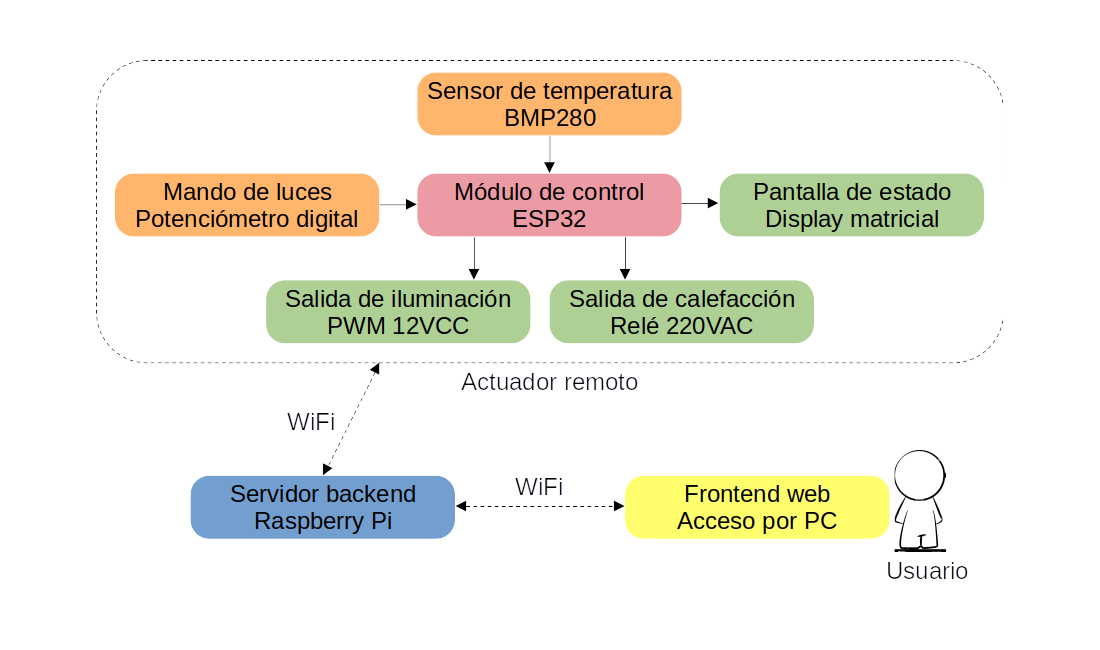
\includegraphics[width=1\textwidth]{./Figuras/Diagrama-bloques.png}
\caption{Diagrama en bloques del sistema.}
\label{fig:diagBloques}
\end{figure}

\vspace{25px}

\section{2. Identificación y análisis de los interesados}
\label{sec:interesados}

\begin{table}[ht]
%\caption{Identificación de los interesados}
%\label{tab:interesados}
\begin{tabularx}{\linewidth}{@{}|l|X|X|l|@{}}
\hline
\rowcolor[HTML]{C0C0C0} 
Rol				& Nombre y Apellido	& Organización		& Puesto 	\\ \hline
%Auspiciante		&					&					&        	\\ \hline
Cliente			& \clientename		&\empclientename		& Especialista de redes IP 	\\ \hline
%Impulsor		&					&					&        	\\ \hline
Responsable		& \authorname		& FIUBA				& Alumno 	\\ \hline
%Colaboradores	&					&					&        	\\ \hline
Orientador		& \supname			& \pertesupname		& Director Trabajo final \\ \hline
Coorientador		& \cosupname			& \pertecosupname	& Codirector Trabajo final \\ \hline
%Equipo			& miembro1 \newline 
%Opositores		&					&					&        	\\ \hline
Usuario final	& Usuarios que habiten o utilicen los recintos	& -		& -       	\\ \hline
\end{tabularx}
\end{table}

\begin{itemize}
	\item Cliente: Mg. Ing. Damián Rubén Corbalán. Es una persona exigente con muchos conocimientos en el tema.
	\item Responsable: Ing. César Javier Fanelli, único responsable a cargo del desarrollo del proyecto. Se ocupará de la planificación y ejecución de las tareas.
	\item Orientador: Ing. Fernando Lichtschein. Debido a su experiencia y conocimiento va a poder colaborar mucho con el desarrollo del proyecto y la resolución de los problemas que surjan en el camino.
\end{itemize}

\section{3. Propósito del proyecto}
\label{sec:proposito}

El propósito de este proyecto es crear un prototipo de sistema de ambientes inteligentes, que sirva como puntapié inicial de un sistema más grande y más completo. Al ser personal la intención es diseñar un sistema que sea potencialmente escalable, al que se le puedan ir agregando más módulos con distintas funcionalidades que sean de utilidad en la vida cotidiana. Dichas funciones futuras podrían ser controlar el acceso (que se lea desde un celular), integrar cámaras de seguridad o sensar y modificar de otros parámetros. El aprendizaje y el desafío son las motivaciones para hacer un proyecto de esta índole. Y si resultara siendo viable técnica y económicamente, en un futuro se analizará la posibilidad de un desarrollo de negocio.

\section{4. Alcance del proyecto}
\label{sec:alcance}

El proyecto en cuestión incluye:
\begin{itemize}
	\item Desarrollo y fabricación de un prototipo de placa que actúe una salida ON-OFF para controlar el calefactor y otra salida para la iluminación.
	\item Desarrollo e implementación de las conexiones entre la placa del punto anterior y la placa de desarrollo con el ESP32 (formando en conjunto el nodo).
	\item Desarrollo del software del nodo.
	\item Desarrollo del software del servidor.
\end{itemize}

El proyecto no incluye:
\begin{itemize}
	\item Otros nodos cuyas funciones no sean las del ejemplo descripto en el diagrama en bloques.
	\item Software en Android o iOS para acceder a la plataforma.
\end{itemize}

\section{5. Supuestos del proyecto}
\label{sec:supuestos}

Para el desarrollo del presente proyecto se supone que:
\begin{itemize}
	\item Se podrán conseguir todos los materiales necesarios para el armado del prototipo.
	\item Se contará con los recursos económicos para desarrollarlo con normalidad.
	\item No surgirán imprevistos personales que retrasen significativamente o pospongan el desarrollo del proyecto o la cursada del posgrado.
	\item Se adquirirán los conocimientos necesarios para la implementación del software y el sistema en su integridad.
	\item Se tendrá apoyo del director en temas netamente técnicos para el desarrollo.
	\item Se tendrá feedback constante del cliente para definir alcance, requerimientos y aprobar la funcionalidad del prototipo.
	\item El cliente cuenta con conexión a Internet y un hardware mínimo para conectar el sistema a su red local.
\end{itemize}

\section{6. Requerimientos}
\label{sec:requerimientos}

Los requerimientos revisados en conjunto con el cliente y agrupados por afinidad son:

\begin{enumerate}
	\item Requerimientos funcionales del sistema.
		\begin{enumerate}
			\item El sistema deberá poder funcionar de forma automática o manual.
			\item El modo automático consistirá en poder programar horarios y niveles de las salidas, seteadas a través de la interfaz web.
			\item El modo manual consistirá en accionar las salidas desde la interfaz web o desde los comandos en el nodo.
			\item Al modificarse de forma manual cualquier parámetro, el nodo informará al servidor el nuevo valor del parámetro seteado.
			\item Al activar el modo manual, se interrumpirá el modo automático.
			\item Se guardarán los valores sensados y seteados en una base de datos dentro del servidor.
			\item Los usuarios podrán revisar los datos de los valores actuales e históricos.
		\end{enumerate}
	\item Requerimientos asociados al nodo.
		\begin{enumerate}
			\item El nodo estará implementado en una placa con un ESP32.
			\item Contará con un potenciómetro digital para elegir la temperatura e iluminación.
			\item Tendrá con un display que mostrará la temperatura sensada y el estado de las salidas.
			\item La frecuencia de sensado de la temperatura será de 1 minuto.
			\item Los niveles de tensión de las entradas y salidas lógicas serán adaptados a los valores lógicos correspondientes de los actuadores.
			\item Se alimentará con una fuente de 5 VCC y un cable microUSB.
		\end{enumerate}
	\item Requerimientos asociados al servidor.
		\begin{enumerate}
			\item El servidor estará montado en una Raspberry Pi con sistema operativo Linux.
			\item Alojará el código de la página web desde la que se ingresará al sistema.
			\item Alojará el código del backend del servidor y la base de datos.
			\item Se alimentará con una fuente de 5 VCC.
		\end{enumerate}
	\item Requerimientos de la interfaz.
		\begin{enumerate}
			\item Será intuitiva y sencilla de operar.
			\item Contará con logueo de usuario y contraseña para ver y cambiar parámetros.
		\end{enumerate}
	\item Requerimientos opcionales (se llevarán a cabo si el tiempo es suficiente).
		\begin{enumerate}
			\item El nodo contará con una salida de dimerización de 220 VCA para ventilación.
			\item El servidor (Raspberry Pi) funcionará como \textit{access point} al que se conectará el nodo.
		\end{enumerate}
\end{enumerate}

\section{7. Historias de usuarios (\textit{Product backlog})}
\label{sec:backlog}

A continuación se enumeran las historias de usuario y se las pondera según la serie de Fibonacci. Los valores elegidos para la dificultad son 3, 5 y 8; para la complejidad 3, 5 y 8 y para la incertidumbre 2, 3 y 5.
\begin{itemize}
	\item Como usuario deseo poder monitorear la temperatura en tiempo real de la habitación para saber si hace falta encender la calefacción. \\
Dificultad: 5 - Complejidad: 3 - Incertidumbre: 3	 - Total: 11 - Valor más cercano 13
	\item Como usuario deseo que el sistema funcione igualmente sin internet para garantizar el confort en la sala. \\
Dificultad: 3 - Complejidad: 3 - Incertidumbre: 2	 - Total: 8 - Valor más cercano 8	
	\item Como usuario quiero que el sistema dé aviso por mail si la temperatura alcanza valores extremos para salvaguardar la integridad de los bienes. \\
Dificultad: 5 - Complejidad: 5 - Incertidumbre: 3	 - Total: 13 - Valor más cercano 13
	\item Como usuario quiero programar la regulación de las luces en horarios programados para simular la presencia de personas en una casa que no está siempre habitada. \\
Dificultad: 5 - Complejidad: 8 - Incertidumbre: 3	 - Total: 16 - Valor más cercano 21
	\item Como usuario quiero almacenar los valores sensados y los estados de las salidas para poder generar un posible ahorro de energía eléctrica. \\
Dificultad: 5 - Complejidad: 5 - Incertidumbre: 3	 - Total: 13 - Valor más cercano 13
	\item Como usuario quiero poder controlar las salidas desde un mando dentro de la habitación para no depender de una PC o teléfono.
Dificultad: 8 - Complejidad: 8 - Incertidumbre: 3	 - Total: 19 - Valor más cercano 21
\end{itemize}

\section{8. Entregables principales del proyecto}
\label{sec:entregables}

Los entregables del proyecto son:

\begin{itemize}
	\item Diagrama de conexión del nodo
	\item Diagrama de circuito esquemático de accesorios del nodo
	\item Código fuente del nodo (ESP32)
	\item Código fuente del frontend y del backend 
	\item Informe final
\end{itemize}

\section{9. Desglose del trabajo en tareas}
\label{sec:wbs}

Las tareas se han agrupado por tema y ordenado por secuencialidad.

\begin{enumerate}
\item Investigación y búsqueda de material (45 h)
	\begin{enumerate}
		\item Búsqueda y análisis de soluciones similares en el mercado (5 h)
		\item Búsqueda de códigos fuente de ejemplo similares (10 h)
		\item Búsqueda y análisis de los materiales a usar (5 h)
		\item Listado de materiales necesarios y aspectos de red (5 h)
		\item Estudio de funcionamiento básico de cada componente del sistema (10 h)
		\item Estudio y diseño de diagrama en bloques del sistema (5 h)
		\item Organizar la documentación y archivar lo importante (5 h)
	\end{enumerate}
\item Adquisición de materiales (15 h)
	\begin{enumerate}
		\item Búsqueda de materiales (3 h)
		\item Análisis de alternativas (2 h)
		\item Armado y análisis de costos (5 h)
		\item Negociación con proveedores y compra de materiales (5 h)
	\end{enumerate}
\item Diseño y puesta en marcha de hardware (85 h)
	\begin{enumerate}
		\item Instalación de sistema operativo Linux en servidor (5 h)
		\item Pruebas de funcionalidad básicas (5 h)
		\item Diseño de circuitos esquemático e impreso del hardware adicional al nodo (10 h)
		\item Armado y pruebas del hardware adicional (20 h)
		\item Conexión y pruebas del hardware adicional con ESP32 (40 h)
		\item Documentar brevemente lo sucedido en este punto (5 h)
	\end{enumerate}
\item Instalación y pruebas de la red local (10 h)
	\begin{enumerate}
		\item Instalación y configuración de la red local (3 h)
		\item Pruebas iniciales de conexión del servidor a la red (2 h)
		\item Pruebas de conexión del nodo a la red (3 h)
		\item Documentar brevemente lo sucedido en este punto (2 h)
	\end{enumerate}
\item Desarrollo del software del servidor (frontend y backend) (292 h)
	\begin{enumerate}
		\item Instalación y configuración del software de la base de datos (5 h)
		\item Instalación y configuración del servidor web (5 h)
		\item Pruebas avanzadas de conexión a la red local e internet (2 h)
		\item Creación del software para la verificación constante de conexión a internet (5 h)
		\item Creación del software para conocer la hora y temperatura local por internet (5 h)
		\item Creación del script para correr los programas automáticamente al encender el servidor (5 h)
		\item Diseño e implementación de la base de datos (10 h)
		\item Diseño y desarrollo de las funcionalidades del backend (40 h)
		\item Pruebas de integración con la base de datos (10 h)
		\item Desarrollo y configuración del código para enviar mails (10 h)
		\item Diseño y maquetación de la página web (20 h)
		\item Desarrollo de la página web (40 h)
		\item Pruebas de funcionalidad de la página web (20 h)
		\item Integración de la página web con el software backend (30 h)
		\item Resolución de problemas de integración (20 h)
		\item Resolución de problemas de funcionamiento (40 h)
		\item Diseño de reportes a presentar por la aplicación (20 h)
		\item Documentar brevemente lo sucedido en este punto (5 h)
	\end{enumerate}
\item Desarrollo del software de nodo (100 h)
	\begin{enumerate}
		\item Diseño de base de software de inicialización y configuración del nodo (5 h)
		\item Diseño de software de lectura de entradas y actuación de salidas (20 h)
		\item Diseño de software de comunicación con el servidor (30 h)
		\item Pruebas de comunicación con el servidor (20 h)
		\item Resolución de problemas (20 h)
		\item Documentar brevemente lo sucedido en este punto (5 h)
	\end{enumerate}
\item Instalación y pruebas funcionales (25 h)
	\begin{enumerate}
		\item Instalación del nodo y adicionales en la habitación (4 h)
		\item Pruebas funcionales de los comandos locales dentro de la habitación (3 h)
		\item Análisis y resolución de posibles fallas (3 h)
		\item Pruebas reales de funcionalidad en un ambiente (5 h)
		\item Pruebas de alarmas y funcionalidad de aplicación web (5 h)
		\item Documentar brevemente lo sucedido en este punto (5 h)
	\end{enumerate}
\item Elaboración de documentación (70 h)
	\begin{enumerate}
		\item Redacción del manual de uso (10 h)
		\item Redacción del informe de avance (10 h)
		\item Elaboración de la memoria técnica (50 h)
	\end{enumerate}
\end{enumerate}

Cantidad total de horas: (642 h). \\
Si en los cálculos anteriores llegara a haber sobrante de tiempo, se puede analizar diseñar e implementar el control de la salida de 220 VCA para controlar la ventilación. Dicha duración de tareas extra (opcionales) se estima de la siguiente manera:
\begin{itemize}

\item Diseño e implementación del control de ventilación mediante salida dimerizable (50 h)
	\begin{enumerate}
		\item Diseño de placa de control de la salida de 220 VCA (10 h)
		\item Armado de placa para dimerizar salida de 220 VCA (10 h)
		\item Conexión al nodo y pruebas (5 h)
		\item Modificación del software del servidor (5 h)
		\item Modificación del software del nodo (20 h)
	\end{enumerate}
\end{itemize}

\section{10. Diagrama de Activity On Node}
\label{sec:AoN}

A continuación se muestra el diagrama \textit{Activity on Node}. Las unidades de tiempo están expresadas en horas (h). El camino crítico está marcado en color rojo. La duración total del camino crítico es de 612 horas.\\
Por la forma de diagramar las tareas en el WBS y al ser el único recurso para hacer todas las actividades, resulta difícil desdoblar la gran mayoría de ellas, por lo que el resultado es el expresado en la imagen.

\begin{figure}[htpb]
\centering 
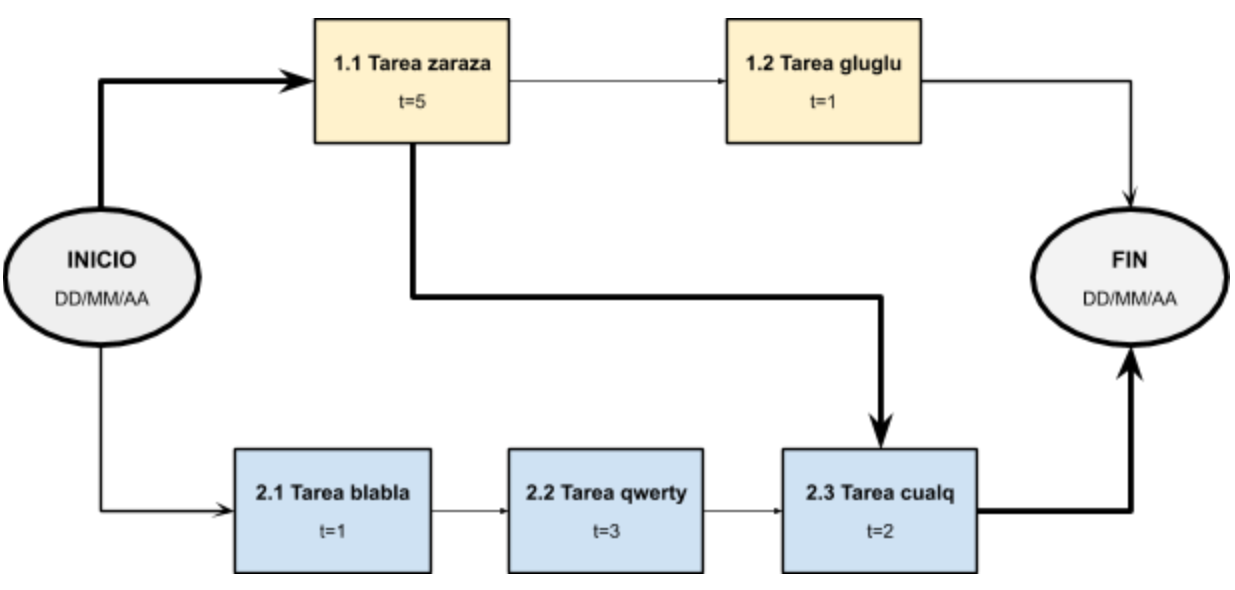
\includegraphics[width=.8\textwidth]{./Figuras/AoN.png}
\caption{Diagrama en \textit{Activity on Node}.}
\label{fig:AoN}
\end{figure}

\section{11. Diagrama de Gantt}
\label{sec:gantt}

A continuación se observa el diagrama de Gantt subdividido en varias partes para que sea legible. La carga horaria semanal promedio se hizo teniendo en cuenta días laborales y días no laborales. En promedio, en días laborales se trabajará 10 horas semanales y en fin de semana se trabajará en promedio 6 horas, dando un total en promedio una carga horaria semanal de 16 hs. Esta carga variará además en base la carga que tengan las materias del posgrado.\\
En la primera imagen se ven los 8 grupos de tareas con la duración total de la realización del proyecto. Luego se ve el desglose en varias imágenes, agrupando las tareas en cuanto a similitud o temas comunes.

\begin{landscape}
\begin{figure}[htpb]
\centering 
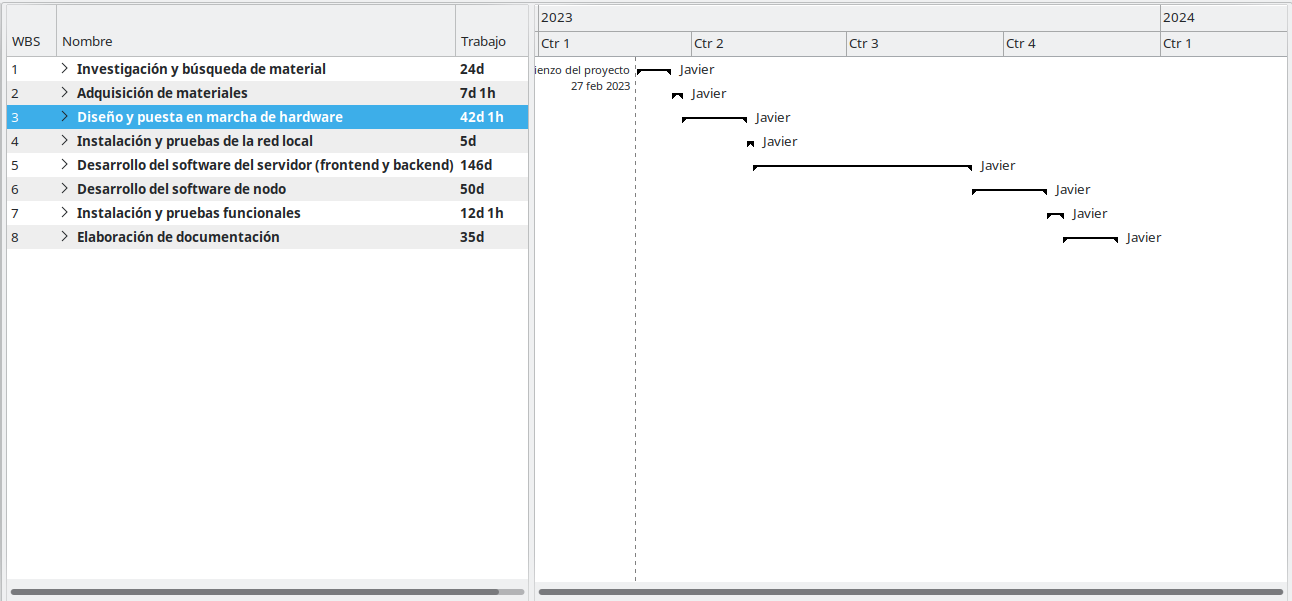
\includegraphics[height=.7\textheight]{./Figuras/Gantt_resumen.png}
\caption{Resumen de gurpos de tareas.}
\label{fig:diagGantt}
\end{figure}
\end{landscape}

\begin{landscape}
\begin{figure}[htpb]
\centering 
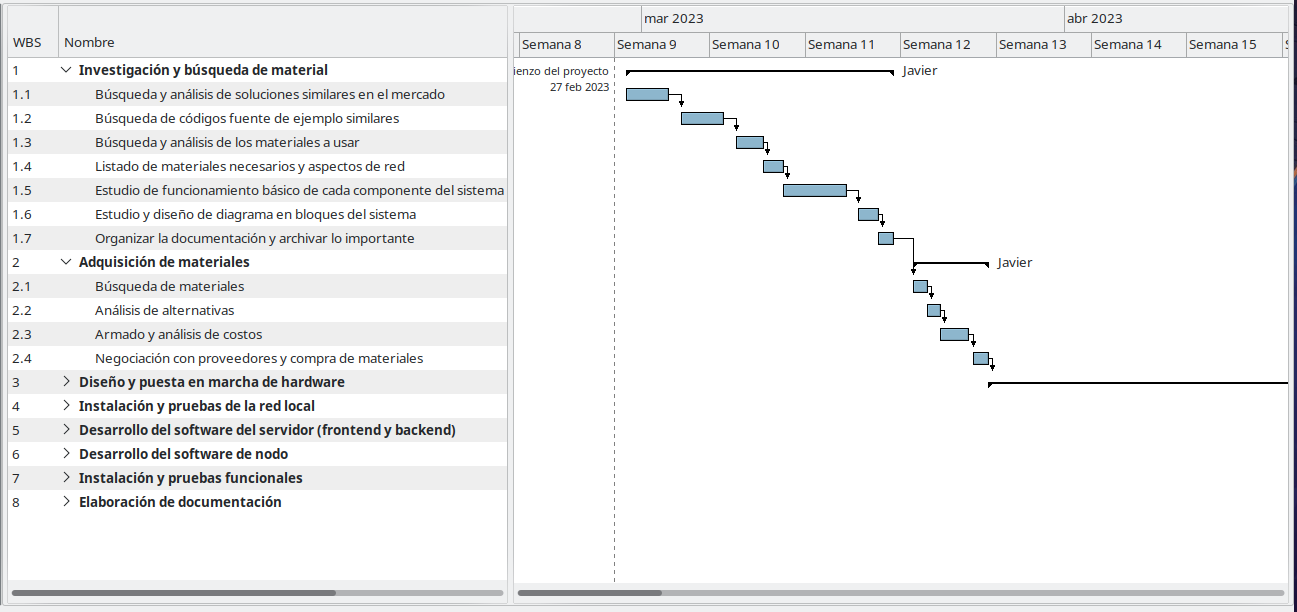
\includegraphics[height=.7\textheight]{./Figuras/Gantt_1-2.png}
\caption{Inicio y pasos preliminares.}
\label{fig:diagGantt}
\end{figure}
\end{landscape}

\begin{landscape}
\begin{figure}[htpb]
\centering 
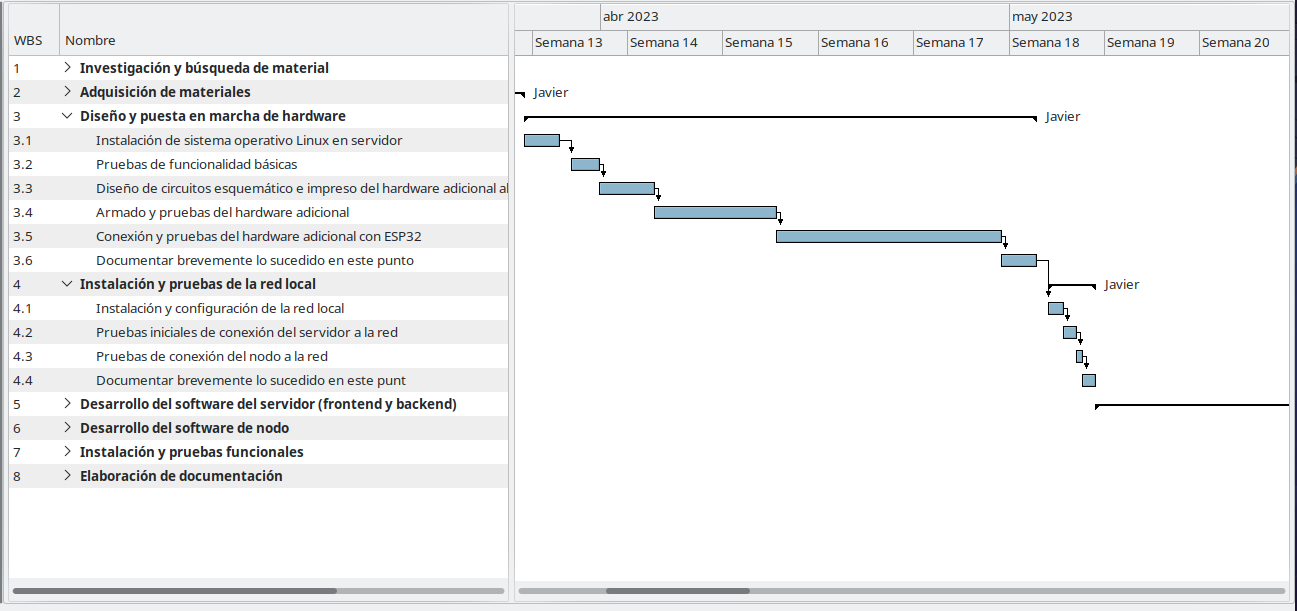
\includegraphics[height=.7\textheight]{./Figuras/Gantt_3-4.png}
\caption{Adecuación del hardware.}
\label{fig:diagGantt}
\end{figure}
\end{landscape}

\begin{landscape}
\begin{figure}[htpb]
\centering 
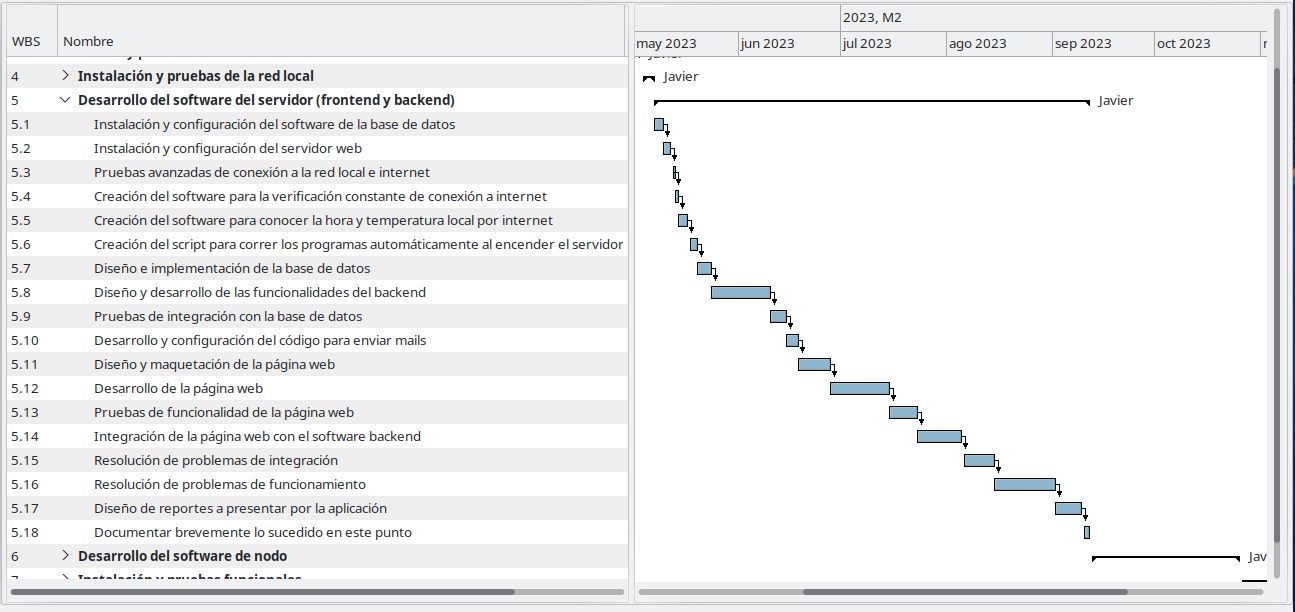
\includegraphics[height=.7\textheight]{./Figuras/Gantt_5.png}
\caption{Desarrollo del software del servidor.}
\label{fig:diagGantt}
\end{figure}
\end{landscape}

\begin{landscape}
\begin{figure}[htpb]
\centering 
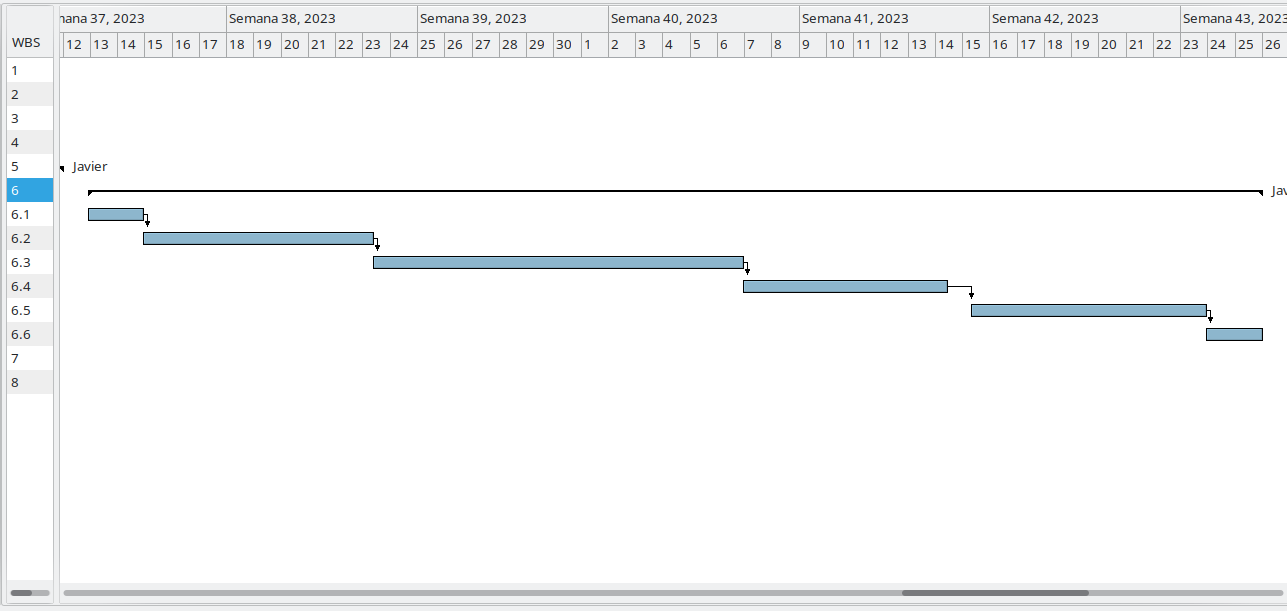
\includegraphics[height=.7\textheight]{./Figuras/Gantt_6.png}
\caption{Desarrollo del software del nodo.}
\label{fig:diagGantt}
\end{figure}
\end{landscape}

\begin{landscape}
\begin{figure}[htpb]
\centering 
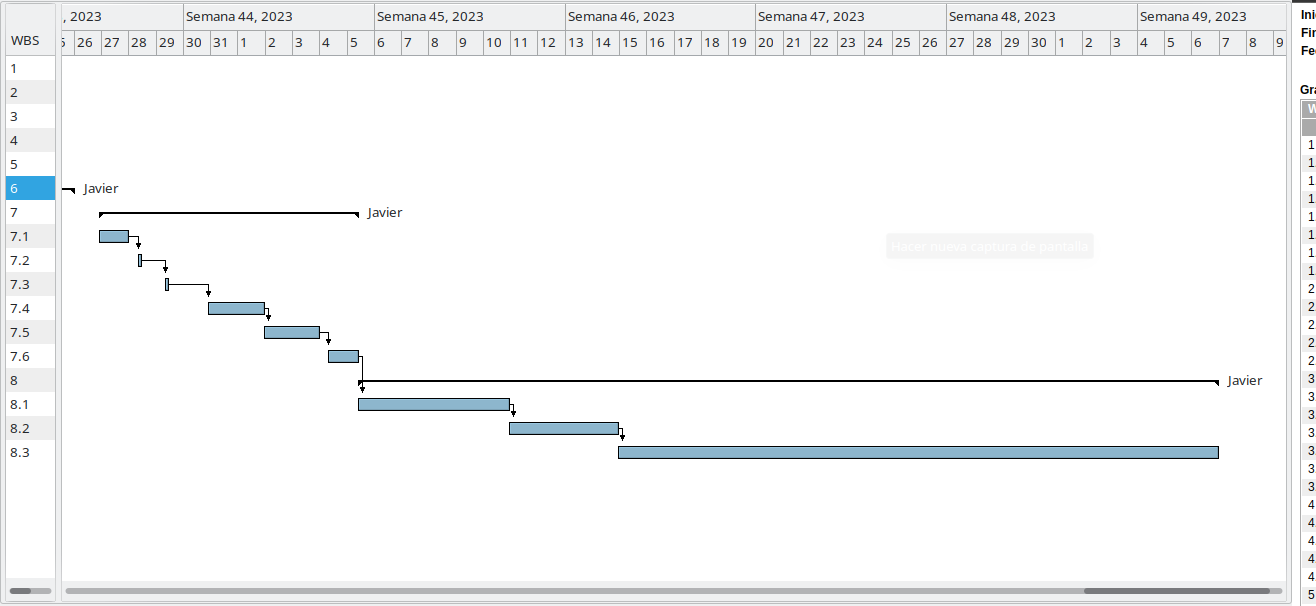
\includegraphics[height=.7\textheight]{./Figuras/Gantt_7-8.png}
\caption{Pruebas finales y desarrollo de documentación.}
\label{fig:diagGantt}
\end{figure}
\end{landscape}

\section{12. Presupuesto detallado del proyecto}
\label{sec:presupuesto}

\begin{table}[htpb]
\centering
\begin{tabularx}{\linewidth}{@{}|X|c|r|r|@{}}
\hline
\rowcolor[HTML]{C0C0C0} 
\multicolumn{4}{|c|}{\cellcolor[HTML]{C0C0C0}COSTOS DIRECTOS} \\ \hline
\rowcolor[HTML]{C0C0C0} 
Descripción &
  \multicolumn{1}{c|}{\cellcolor[HTML]{C0C0C0}Cantidad} &
  \multicolumn{1}{c|}{\cellcolor[HTML]{C0C0C0}Valor unitario} &
  \multicolumn{1}{c|}{\cellcolor[HTML]{C0C0C0}Valor total} \\ \hline
Placa desarrollo ESP32C3 &
  \multicolumn{1}{c|}{1} &
  \multicolumn{1}{c|}{\$7239} &
  \multicolumn{1}{c|}{\$7239} \\ \hline
Display Oled 1.3 pulgadas Azul 128x64 I2C &
  \multicolumn{1}{c|}{1} &
  \multicolumn{1}{c|}{\$2685} &
  \multicolumn{1}{c|}{\$2685} \\ \hline
Encoder rotativo con pulsador &
  \multicolumn{1}{c|}{1} &
  \multicolumn{1}{c|}{\$360} &
  \multicolumn{1}{c|}{\$360} \\ \hline
Placa experimental perforada simple faz 7x9 cm &
  \multicolumn{1}{c|}{2} &
  \multicolumn{1}{c|}{\$779} &
  \multicolumn{1}{c|}{\$1558} \\ \hline
Sensor de presión y temperatura I2C BMP280 &
  \multicolumn{1}{c|}{1} &
  \multicolumn{1}{c|}{\$404} &
  \multicolumn{1}{c|}{\$404} \\ \hline
Cables, conectores y componentes genéricos &
  \multicolumn{1}{c|}{1} &
  \multicolumn{1}{c|}{\$2500} &
  \multicolumn{1}{c|}{\$2500} \\ \hline
Fuente 5 VCC 500 mA miniUSB &
  \multicolumn{1}{c|}{1} &
  \multicolumn{1}{c|}{\$500} &
  \multicolumn{1}{c|}{\$500} \\ \hline
Raspberry Pi 4 Model B 4 GB &
  \multicolumn{1}{c|}{1} &
  \multicolumn{1}{c|}{\$80000} &
  \multicolumn{1}{c|}{\$80000} \\ \hline
Fuente 5 VCC 3000 mA USB-C &
  \multicolumn{1}{c|}{1} &
  \multicolumn{1}{c|}{\$500} &
  \multicolumn{1}{c|}{\$500} \\ \hline
Memoria Micro SD 32 GB 100 MB/s &
  \multicolumn{1}{c|}{1} &
  \multicolumn{1}{c|}{\$3500} &
  \multicolumn{1}{c|}{\$3500} \\ \hline
    
\multicolumn{3}{|c|}{SUBTOTAL} &
  \multicolumn{1}{c|}{\$99246} \\ \hline
\rowcolor[HTML]{C0C0C0} 
\multicolumn{4}{|c|}{\cellcolor[HTML]{C0C0C0}COSTOS INDIRECTOS} \\ \hline
\rowcolor[HTML]{C0C0C0} 
Descripción &
	\multicolumn{1}{c|}{\cellcolor[HTML]{C0C0C0}Cantidad} &
	\multicolumn{1}{c|}{\cellcolor[HTML]{C0C0C0}Valor unitario} &
	\multicolumn{1}{c|}{\cellcolor[HTML]{C0C0C0}Valor total} \\ \hline
\multicolumn{1}{|l|}{40\% de los costos directos} & 1
   & \$39098
   & \$39098
   \\ \hline

\multicolumn{3}{|c|}{SUBTOTAL} &
  \multicolumn{1}{c|}{\$39098} \\ \hline
\rowcolor[HTML]{C0C0C0}
\multicolumn{3}{|c|}{TOTAL} & \$138344
   \\ \hline
\end{tabularx}%
\end{table}
El presupuesto anterior da un total estimado de \$138344. Ante el escenario inflacionario actual los precios varían mes a mes, por lo que se estima el presupuesto en dólares. Tomando un valor de \$169 por dólar al 17/11/2022, el mismo da un estimado de USD818,60.

\section{13. Gestión de riesgos}
\label{sec:riesgos}

a) Identificación de los riesgos y estimación de sus ocurrencias.

Los riesgos listados a continuación son ponderados del 1 al 10 en severidad (S) y probabilidad de ocurrencia (O).
 
Riesgo 1: desabastecimiento de componentes claves del sistema.
\begin{itemize}
	\item Severidad (8): de no conseguir los componentes más importantes del sistema habrá que buscar opciones y re adaptar parte del código, lo cual introduciría demoras.
	\item Ocurrencia (7): hay escasez a nivel mundial las placas Raspberry Pi y Argentina está en un período de dificultades con las importaciones.
\end{itemize}   

Riesgo 2: incompatibilidad del hardware adicional con la placa del ESP32.
\begin{itemize}
	\item Severidad (4): el hardware no funciona de la manera esperada por incompatibilidad entre las tensiones, corrientes o frecuencias.
	\item Ocurrencia (4): se tiene experiencia previa en desarrollo de hardware similar y son problemas frecuentes.
\end{itemize}

Riesgo 3: demoras en el desarrollo del software del servidor.
\begin{itemize}
	\item Severidad (7): es el software con más carga de trabajo a realizar y más complejo del sistema y sin este no hay funcionalidad en una plataforma de IoT.
	\item Ocurrencia (7): no se tiene la experiencia necesaria al momento del desarrollo del presente documento para hacer la tarea en su totalidad.
\end{itemize}

Riesgo 4: problemas de comunicación entre el nodo y el servidor.
\begin{itemize}
	\item Severidad (6): si bien el nodo podrá programarse de forma local, perdería la capacidad de tomar parámetros pasados de forma remota y el servidor perdería los parámetros que está sensando el nodo.
	\item Ocurrencia (4): al ser programados en plataformas y lenguajes distintos, es probable que haya problemas de envío o interpretación de datos.
\end{itemize}

Riesgo 5: inestabilidad en la conexión con la red.
\begin{itemize}
	\item Severidad (5): la conexión del nodo a la red es indispensable para poder leer las entradas y modificar las salidas.
	\item Ocurrencia (3): al estar conectado de forma inalámbrica puede ser que la señal de \textit{Wi-Fi} sea débil en la ubicación del nodo.
\end{itemize}

Riesgo 6: daño de la tarjeta de memoria del servidor.
\begin{itemize}
	\item Severidad (9): en la tarjeta de memoria de la Raspberry Pi se guardan todos los datos tomados, corre el sistema operativo y todo el software desarrollado en el proyecto.
	\item Ocurrencia (4): al tener varias lecturas y escrituras se corre el riesgo de que se fatigue la memoria micro SD y se pierda la información.
\end{itemize}

Riesgo 7: imposibilidad de hacer una instalación básica para pruebas.
\begin{itemize}
	\item Severidad (8): sin una instalación básica de pruebas no se puede hacer la depuración completa del prototipo.
	\item Ocurrencia (2): las instalaciones se pueden hacer en lugares de forma básica y hasta en una maqueta.
\end{itemize}

b) Tabla de gestión de riesgos (El RPN se calcula como RPN=SxO).

\begin{table}[htpb]
\centering
\begin{tabularx}{\linewidth}{@{}|X|c|c|c|c|c|c|@{}}
\hline
\rowcolor[HTML]{C0C0C0} 
Riesgo & S & O & RPN & S* & O* & RPN* \\ \hline
1. Desabastecimiento de componentes claves del sistema				&8	&7	&56\cellcolor{red}	&8	&2	&16\cellcolor{green}	\\ \hline
2. Incompatibilidad del hardware adicional con la placa del ESP32	&4	&4	&16\cellcolor{green}	&	&	&	\\ \hline
3. Demoras en el desarrollo del software del servidor				&7	&7	&49\cellcolor{red}	&7	&3	&21\cellcolor{green} 	\\ \hline
4. Problemas de comunicación entre el nodo y el servidor				&6	&4	&24\cellcolor{green}	&	&	& 	\\ \hline
5. Inestabilidad en la conexión con la red							&5	&3	&15\cellcolor{green}	&	&	&	\\ \hline
6. Daño de la tarjeta de memoria del servidor						&9	&4	&36\cellcolor{red}	&3	&4	&12\cellcolor{green}	\\ \hline
7. Imposibilidad de hacer una instalación básica para pruebas		&8	&2	&16\cellcolor{green}	&	&	&	\\ \hline
\end{tabularx}%
\end{table}

Criterio adoptado: se tomarán medidas de mitigación en los riesgos cuyos números de RPN sean mayores a 25 puntos.
Nota: los valores marcados con (*) en la tabla corresponden luego de haber aplicado la mitigación.

c) Plan de mitigación de los riesgos que originalmente excedían el RPN máximo establecido.
 
Riesgo 1: desabastecimiento de componentes claves del sistema.
\begin{itemize}
	\item Plan de mitigación: adelantar las compras para cuando se tenga tiempo y los recursos materiales.
	\item Severidad* (8): la severidad sigue siendo la misma, ya que si no se dispone del hardware no se puede desarrollar el prototipo para el proyecto.
	\item Ocurrencia* (2): hacia fines del 2022 todavía hay stock de la placa Raspberry Pi y ESP32, por lo que se planea hacerlo en breve.
\end{itemize}
  
Riesgo 3: demoras en el desarrollo del software del servidor.
\begin{itemize}
	\item Plan de mitigación: se buscará información y se capacitará, se comenzarán con pruebas previas al desarrollo del proyecto durante los meses diciembre, enero y febrero previos al inicio del desarrollo del proyecto.
	\item Severidad* (7): la severidad sigue siendo la misma ya que por más que se adelanten tareas, sin este desarrollo el sistema no es de IoT.
	\item Ocurrencia* (3): al adelantar la adquisición de algunos conocimientos, los preparativos del entorno de la Raspberry Pi y probablemente alguna parte del código bajan las chances de sufrir demoras.
\end{itemize}

Riesgo 6: daño de la tarjeta de memoria del servidor.
\begin{itemize}
	\item Plan de mitigación: se harán backups cada semana o cambio importante de la información creada y código desarrollado, y se creará una imagen de la memoria.
	\item Severidad* (3): se disminuye la severidad ya que si se dañara o se perdiera información el único perjuicio es incurrir en una demora para la recuperación de la información.
	\item Ocurrencia* (4): la probabilidad de ocurrencia es la misma ya que puede pasar de igual manera, y se trabaja en mitigar la severidad del riesgo creando copias.
\end{itemize}

\section{14. Gestión de la calidad}
\label{sec:calidad}

\begin{enumerate}
	\item Requerimientos funcionales del sistema.
		\begin{enumerate}
			\item El sistema deberá poder funcionar de forma automática o manual.
			\begin{itemize}
				\item Verificación: se creará el software con 2 modos, incluyendo un script para conocer la hora local y adicionando al nodo hardware para la modificación de parámetros.
				\item Validación: se validará la existencia de los modos desde la aplicación web.
			\end{itemize}
			\item El modo automático consistirá en poder programar horarios y niveles de las salidas, seteadas a través de la interfaz web.
			\begin{itemize}
				\item Verificación: se incorporará un script para saber la hora local al software y se programarán funciones con horarios.
				\item Validación: a través de la interfaz web se crearán funciones con horarios y se validará el accionamiento de las salidas.
			\end{itemize}
			\item El modo manual consistirá en accionar las salidas desde la interfaz web o desde los comandos en el nodo.
			\begin{itemize}
				\item Verificación: se analizarán las hojas de datos del ESP32 y del hardware utilizado realizando pruebas funcionales.
				\item Validación: se accionarán los controles del nodo modificando los parámetros, validando el cambio de las salidas.
			\end{itemize}
			\item Al modificarse de forma manual cualquier parámetro, el nodo informará al servidor el nuevo valor del parámetro seteado.
			\begin{itemize}
				\item Verificación: se incorporará una función de envío de parámetros dentro del software del nodo y se verificará el envío de datos.
				\item Validación: se accionarán los controles viendo al mismo tiempo que se modifiquen en la aplicación web.
			\end{itemize}
			\item Al activar el modo manual, se interrumpirá el modo automático.
			\begin{itemize}
				\item Verificación: se incorporará una función en el backend para que dé aviso al nodo el cambio del modo a automático y se verificará el envío de datos.
				\item Validación: se activará el modo automático cargándole funciones y se validará de cambio del modo en el nodo.
			\end{itemize}
			\item Se guardarán los valores sensados y seteados en una base de datos dentro del servidor.
			\begin{itemize}
				\item Verificación: se verificará el envío periódico de datos del nodo al servidor informando el estado de las salidas y los sensores conectados y muestra de estos valores.
				\item Validación: se validará mediante la muestra de los valores en tiempo real en la aplicación web.
			\end{itemize}
			\item Los usuarios podrán revisar los datos de los valores actuales e históricos.
			\begin{itemize}
				\item Verificación: se incorporará una base de datos en el servidor que almacene los parámetros y se verificará la cantidad y calidad de estos datos.
				\item Validación: se presentarán en pantalla a través de la aplicación web los parámetros almacenados en la base de datos.
			\end{itemize}
		\end{enumerate}
	\item Requerimientos asociados al nodo.
		\begin{enumerate}
			\item El nodo estará implementado en una placa con un ESP32.
			\begin{itemize}
				\item Verificación: se estudiarán los aspectos necesarios en las hojas de datos de la placa ESP32.
				\item Validación: se adjuntarán imágenes del nodo con la placa conectada dentro de él.
			\end{itemize}
			\item Contará con un potenciómetro digital para elegir la temperatura e iluminación.
			\begin{itemize}
				\item Verificación: se estudiarán las hojas de datos del potenciómetro, se medirá con osciloscopio o similar y se verificará el funcionamiento en placa de prueba.
				\item Validación: se accionará el potenciómetro para modificar parámetros y poder observar las variaciones.
			\end{itemize}
			\item Tendrá con un display que mostrará la temperatura sensada y el estado de las salidas.
			\begin{itemize}
				\item Verificación: se estudiarán las hojas de datos del display y se verificará que se muestren los datos.
				\item Validación: se mostrará la lectura de pantalla con información y corroboración visual del estado de las salidas.
			\end{itemize}
			\item La frecuencia de sensado de la temperatura será de 1 minuto.
			\begin{itemize}
				\item Verificación: se programará el software del nodo para tomar lectura de los sensores canda un minuto usando timers internos y se verificará el envío de datos en ese intervalo de tiempo.
				\item Validación: se mostrarán los datos sensados en la pantalla del nodo y en la aplicación web, actualizándose con cada lectura y envío de información.
			\end{itemize}
			\item Los niveles de tensión de las entradas y salidas lógicas serán adaptados a los valores lógicos correspondientes de los actuadores.
			\begin{itemize}
				\item Verificación: se utilizarán transistores bipolares o FET para conmutar las salidas de la placa del ESP32. Se verificarán las hojas de datos de todos los componentes.
				\item Validación: se detectará y mostrará el accionamiento correcto de las salidas.
			\end{itemize}
			\item Se alimentará con una fuente de 5 VCC y un cable microUSB.
			\begin{itemize}
				\item Verificación: se estudiarán las hojas de datos de la placa del ESP32.
				\item Validación: se validará el encendido y correcto funcionamiento.
			\end{itemize}
		\end{enumerate}
	\item Requerimientos asociados al servidor.
		\begin{enumerate}
			\item El servidor estará montado en una Raspberry Pi con sistema operativo Linux.
			\begin{itemize}
				\item Verificación: se comprobará el funcionamiento del sistema operativo con conexión a una pantalla y se harán algunas pruebas de software.
				\item Validación: se adjuntarán imágenes del hardware del servidor.
			\end{itemize}
			\item Alojará el código de la página web desde la que se ingresará al sistema.
			\begin{itemize}
				\item Verificación: se desarrollará el software frontend dentro de la memoria que alojará la Raspberry Pi.
				\item Validación: se mostrará el encendido del servidor y se accederá a la aplicación web.
			\end{itemize}
			\item Alojará el código del backend del servidor y la base de datos.
			\begin{itemize}
				\item Verificación: se desarrollará el software backend dentro de la memoria que alojará la Raspberry Pi.
				\item Validación: se comprobarán los datos recopilados y guardados en la base de datos.
			\end{itemize}
			\item Se alimentará con una fuente de 5 VCC.
			\begin{itemize}
				\item Verificación: se estudiarán las hojas de datos de la Raspberry Pi.
				\item Validación: se mostrará un esquema de conexión del hardware del servidor.
			\end{itemize}
		\end{enumerate}
	\item Requerimientos de la interfaz.
		\begin{enumerate}
			\item Será intuitiva y sencilla de operar.
			\begin{itemize}
				\item Verificación: se desarrollará la aplicación web en base a experiencias de usuario y se harán pruebas funcionales con clientes potenciales.
				\item Validación: se demostrará la aplicación web dando un breve recorrido y explicación y se escucharán sugerencias y reclamos.
			\end{itemize}
			\item Contará con logueo de usuario y contraseña para ver y cambiar parámetros.
			\begin{itemize}
				\item Verificación: se desarrollará y probará el frontend y del backend con un usuario y clave.
				\item Validación: se creará de un usuario para que el cliente pueda ver los estados y datos almacenados.
			\end{itemize}
		\end{enumerate}
\end{enumerate}

\section{15. Procesos de cierre}    
\label{sec:cierre}

\begin{itemize}
	\item Análisis de las pautas de trabajo del desarrollo del Plan de Proyecto.
	\begin{itemize}	
		\item Responsable: Ing. César Javier Fanelli.
		\item Participación: Mg. Ing. Damián Rubén Corbalán (cliente).
	\end{itemize}	
	En este proceso se analizarán: el cumplimiento los requerimientos y los entregables en conjunto con el cliente; que se haya respetado la fecha de entrega y si hubo desvíos en la duración de las tareas con respecto al diagrama de Gantt planteado; la eficiencia de recursos utilizados y su hubo desvíos en el presupuesto presentado en el plan y su justificación.
	\item Análisis de técnicas y procedimientos durante el desarrollo del proyecto.
	\begin{itemize}	
		\item Responsable: Ing. César Javier Fanelli.
		\item Participación: Ing. Fernando Lichtschein (director del trabajo final).
	\end{itemize}
	En este proceso se analizarán las técnicas de programación, lenguajes utilizados, estructura de la base de datos, protocolos de comunicación, diseño de los circuitos anexos y la resolución de problemas que surgieron en el desarrollo. Se pedirá opinión al director del proyecto que con su experiencia podrá aportar otro enfoque.
	\item Defensa pública del proyecto.
	\begin{itemize}	
		\item Responsable: Ing. César Javier Fanelli.
	\end{itemize}
	Se llevará a cabo de forma virtual y participarán los interesados, jurados y autoridades de la especialización.Al final de la presentación se agradecerá formalmente a todos aquellos que
colaboraron durante el proyecto.
\end{itemize}

\end{document}
